\chapter{Holding}
\label{ch:holding}

Safe and effective prescribed fire begins with good \emph{control lines}\textemdash ``an inclusive term for all constructed or natural barriers and treated fire edges used to control a fire.\citep{nwcg2019}.'' \footnote{Managers (and this text) often use ``firebreak'', ``control line'', and ``fire line'' interchangeably, although this last term is more specific to line constructed for indirect attack of wildfire. }
While in wildfire suppression operations control lines are often hurriedly established in response to an ignition and anticipated direction of spread, prescribed fire managers have the advantage of defining the spatial extent of fire on their own terms. 

No control line can guarantee success on its own. 
But thoughtfully-placed and appropriately developed control lines provide a strong foundation to start fires with a high probability of remaining within the burn unit while affording managers good sight lines and accessibility. 

\section{Types of firebreaks}

\begin{figure}
	\begin{center}
		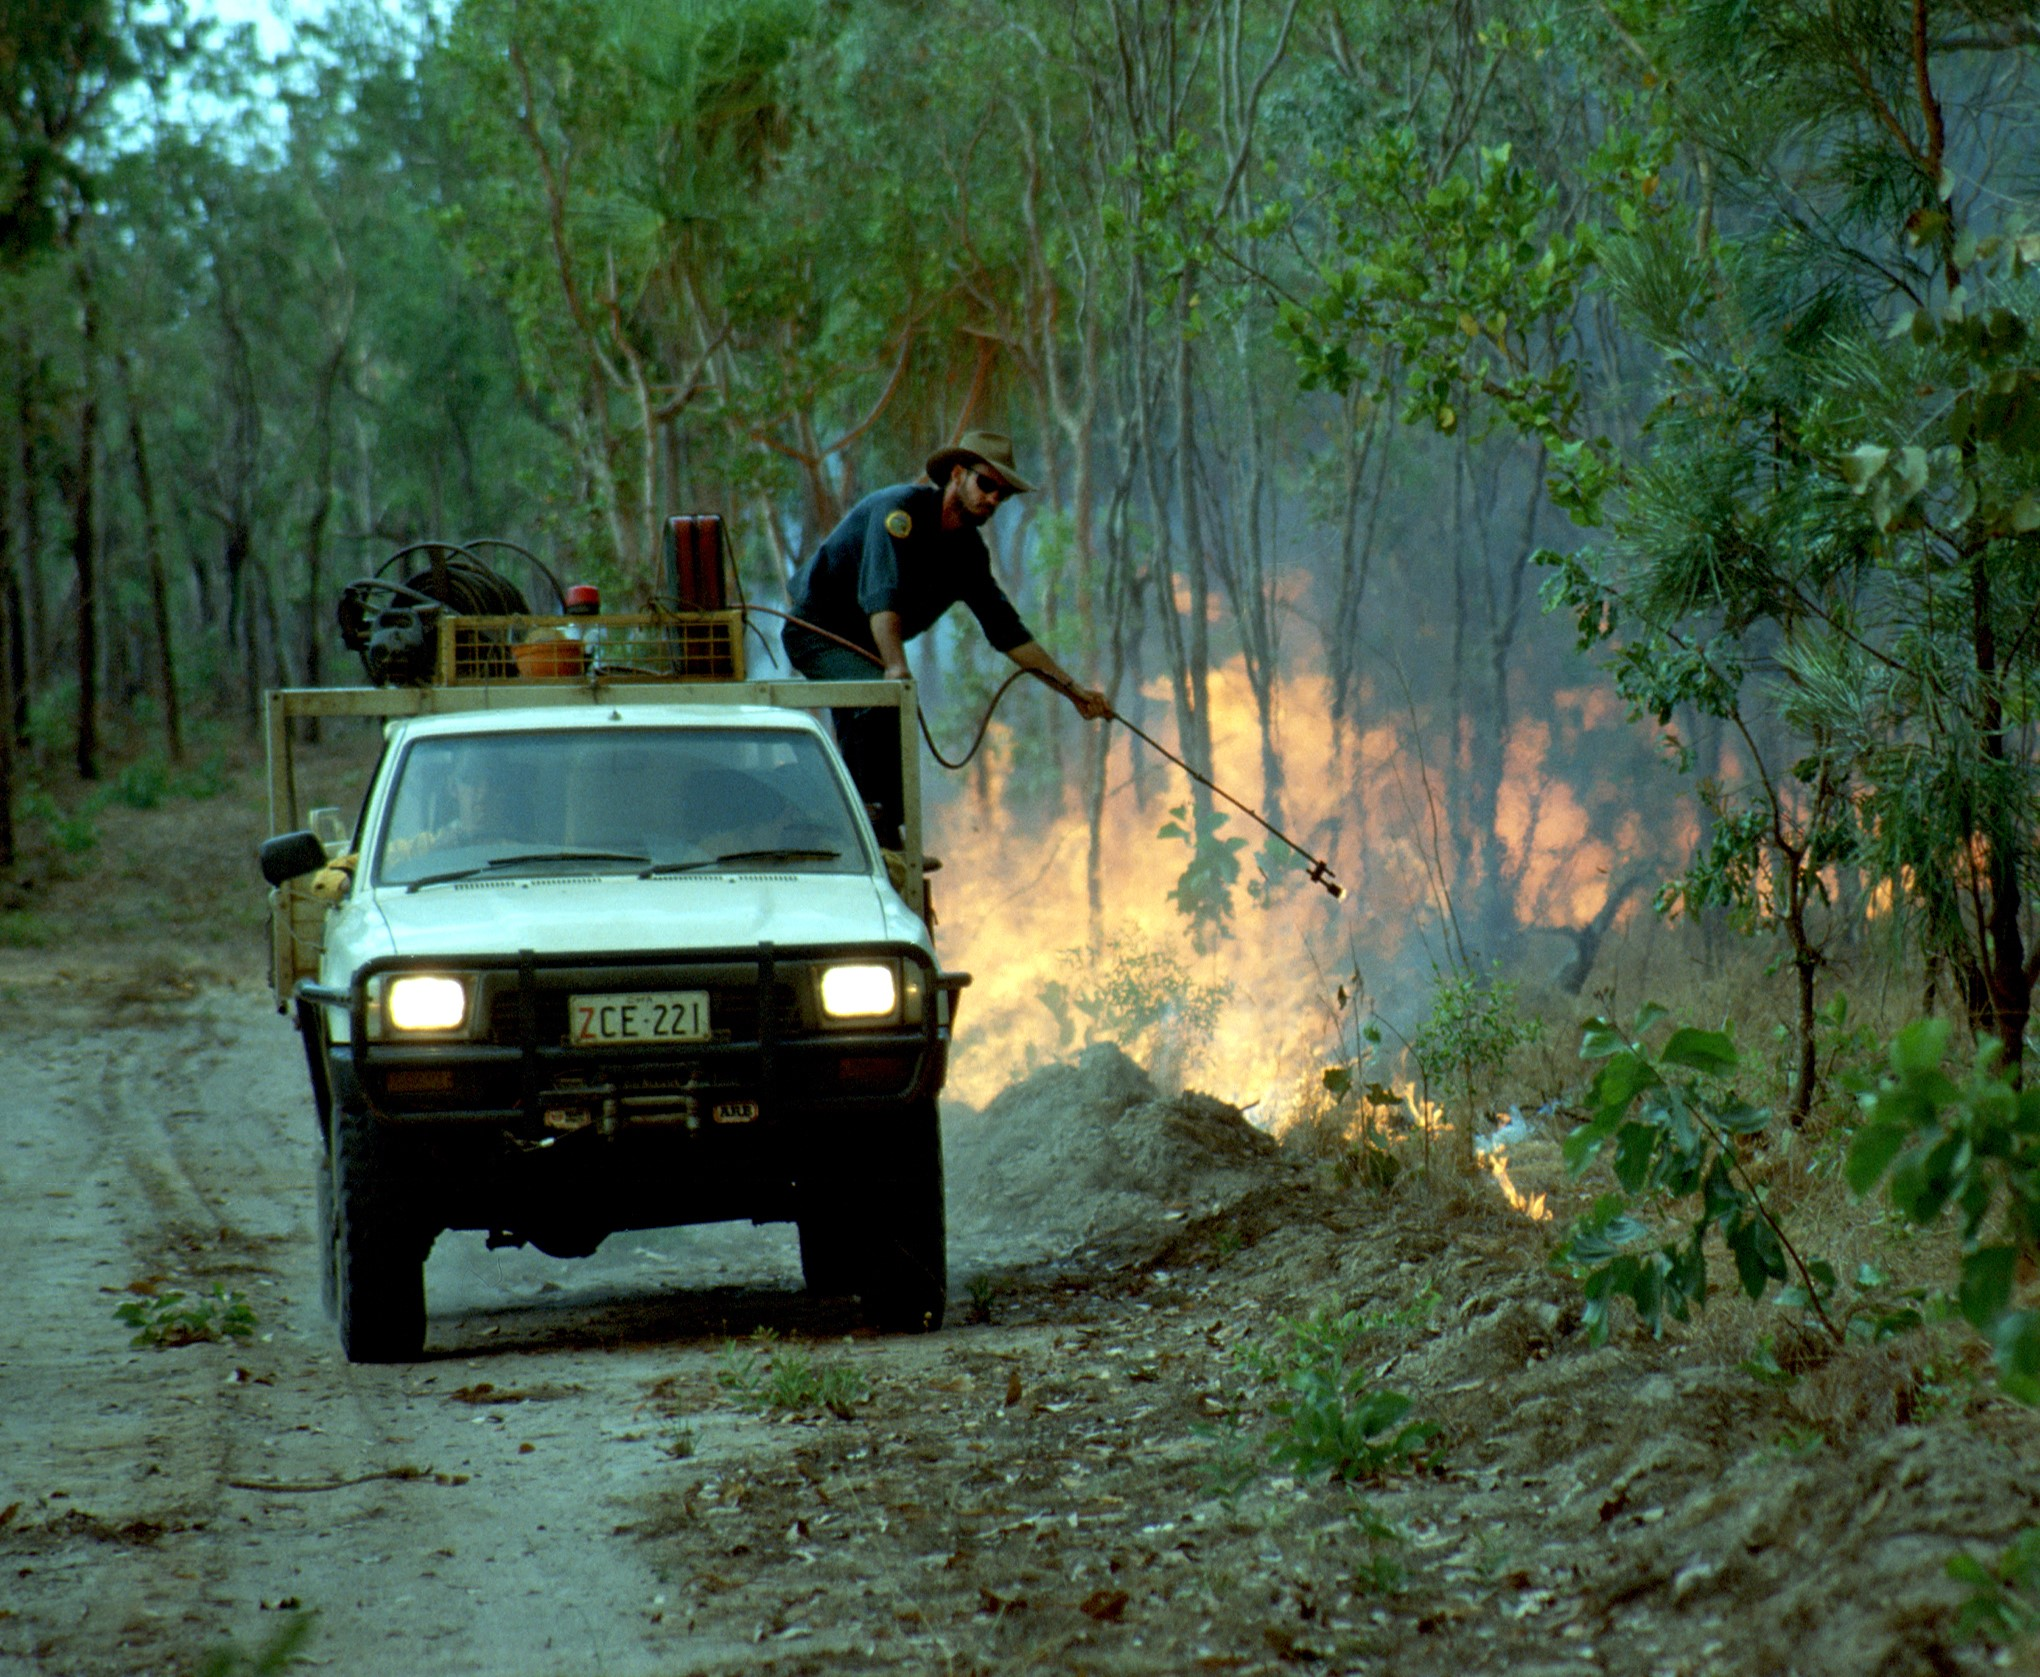
\includegraphics[width=0.45\textwidth]
		{ops/holding/DA0225}~
		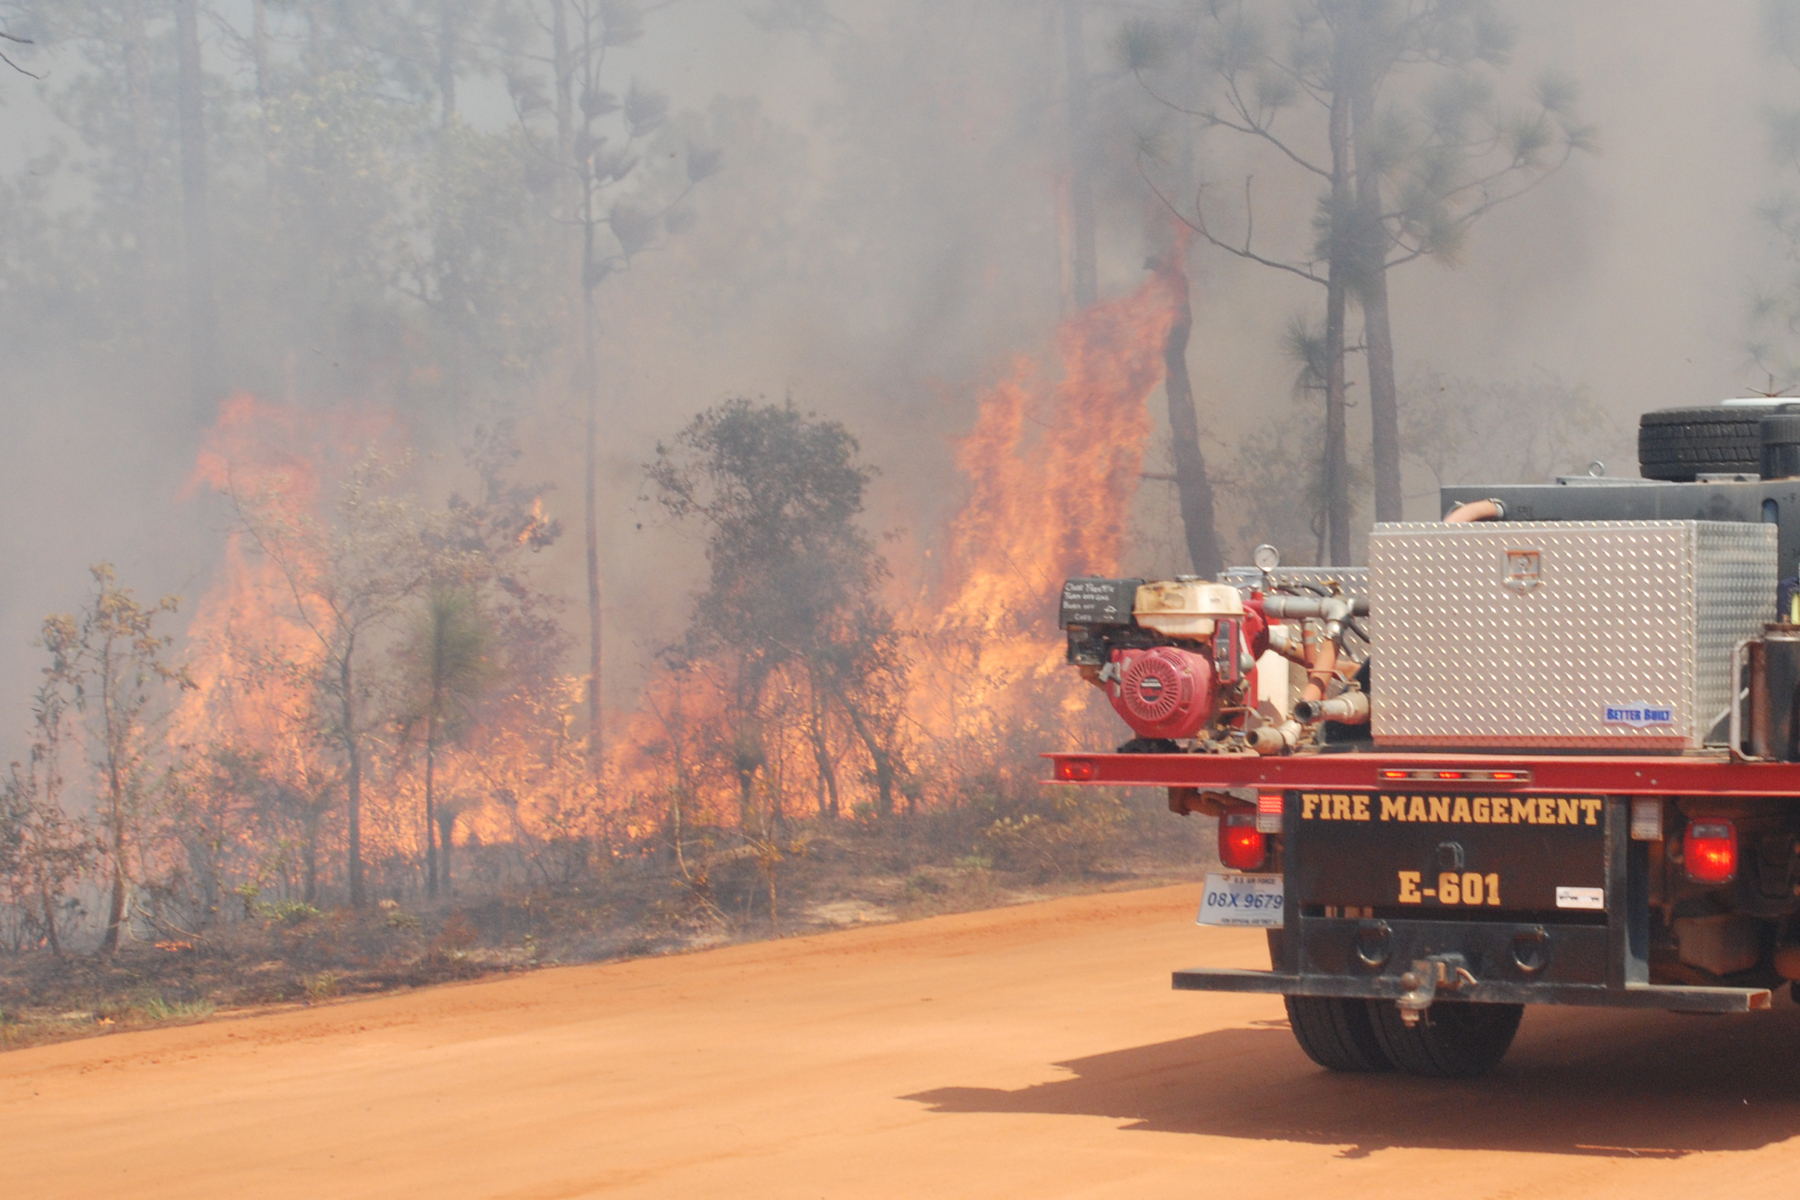
\includegraphics[width=0.55\textwidth]
		{ops/holding/GravelRoadBreak} \\ 
		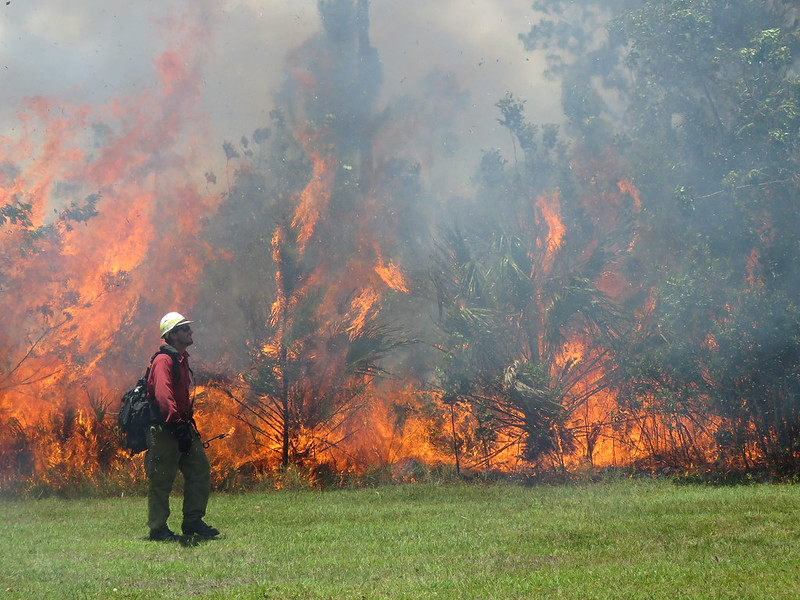
\includegraphics[width=0.47\textwidth]
		{ops/holding/HoldingEmberWatchOut}~
		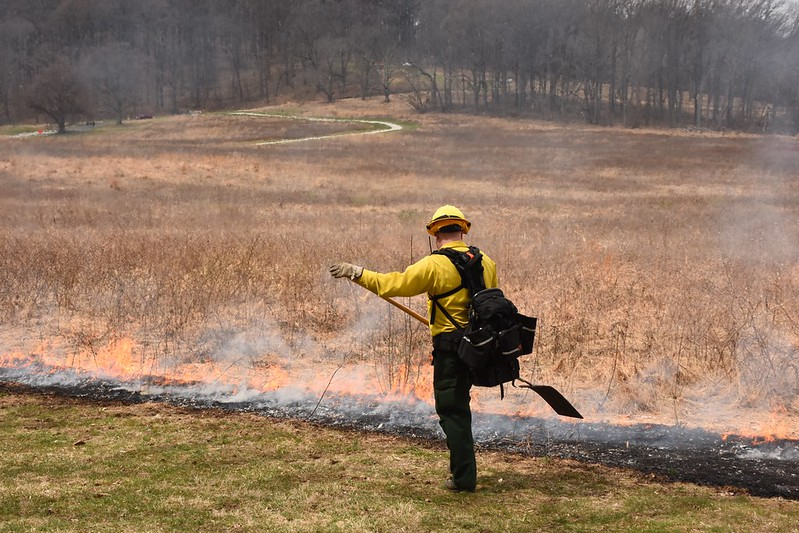
\includegraphics[width=0.53\textwidth]
		{ops/holding/FlapperHolding}
	\end{center}
	\caption{Examples of readymade fire breaks.
		\emph{Top:} Existing roads make good firebreaks\textemdash typically wide, non-flammable, and accessible to equipment for ignition, holding, and suppression. 
		\emph{Bottom:} Two firefighters attend to fires from low-load, high-moisture vegetation conducive to containment. 
	} \label{fig:ReadyMadeBreaks}
	%(Fig.~\ref{fig:ReadyMadeBreaks})
\end{figure}

\subsection{Readymade breaks} 

 \begin{marginfigure}
	\begin{center}
		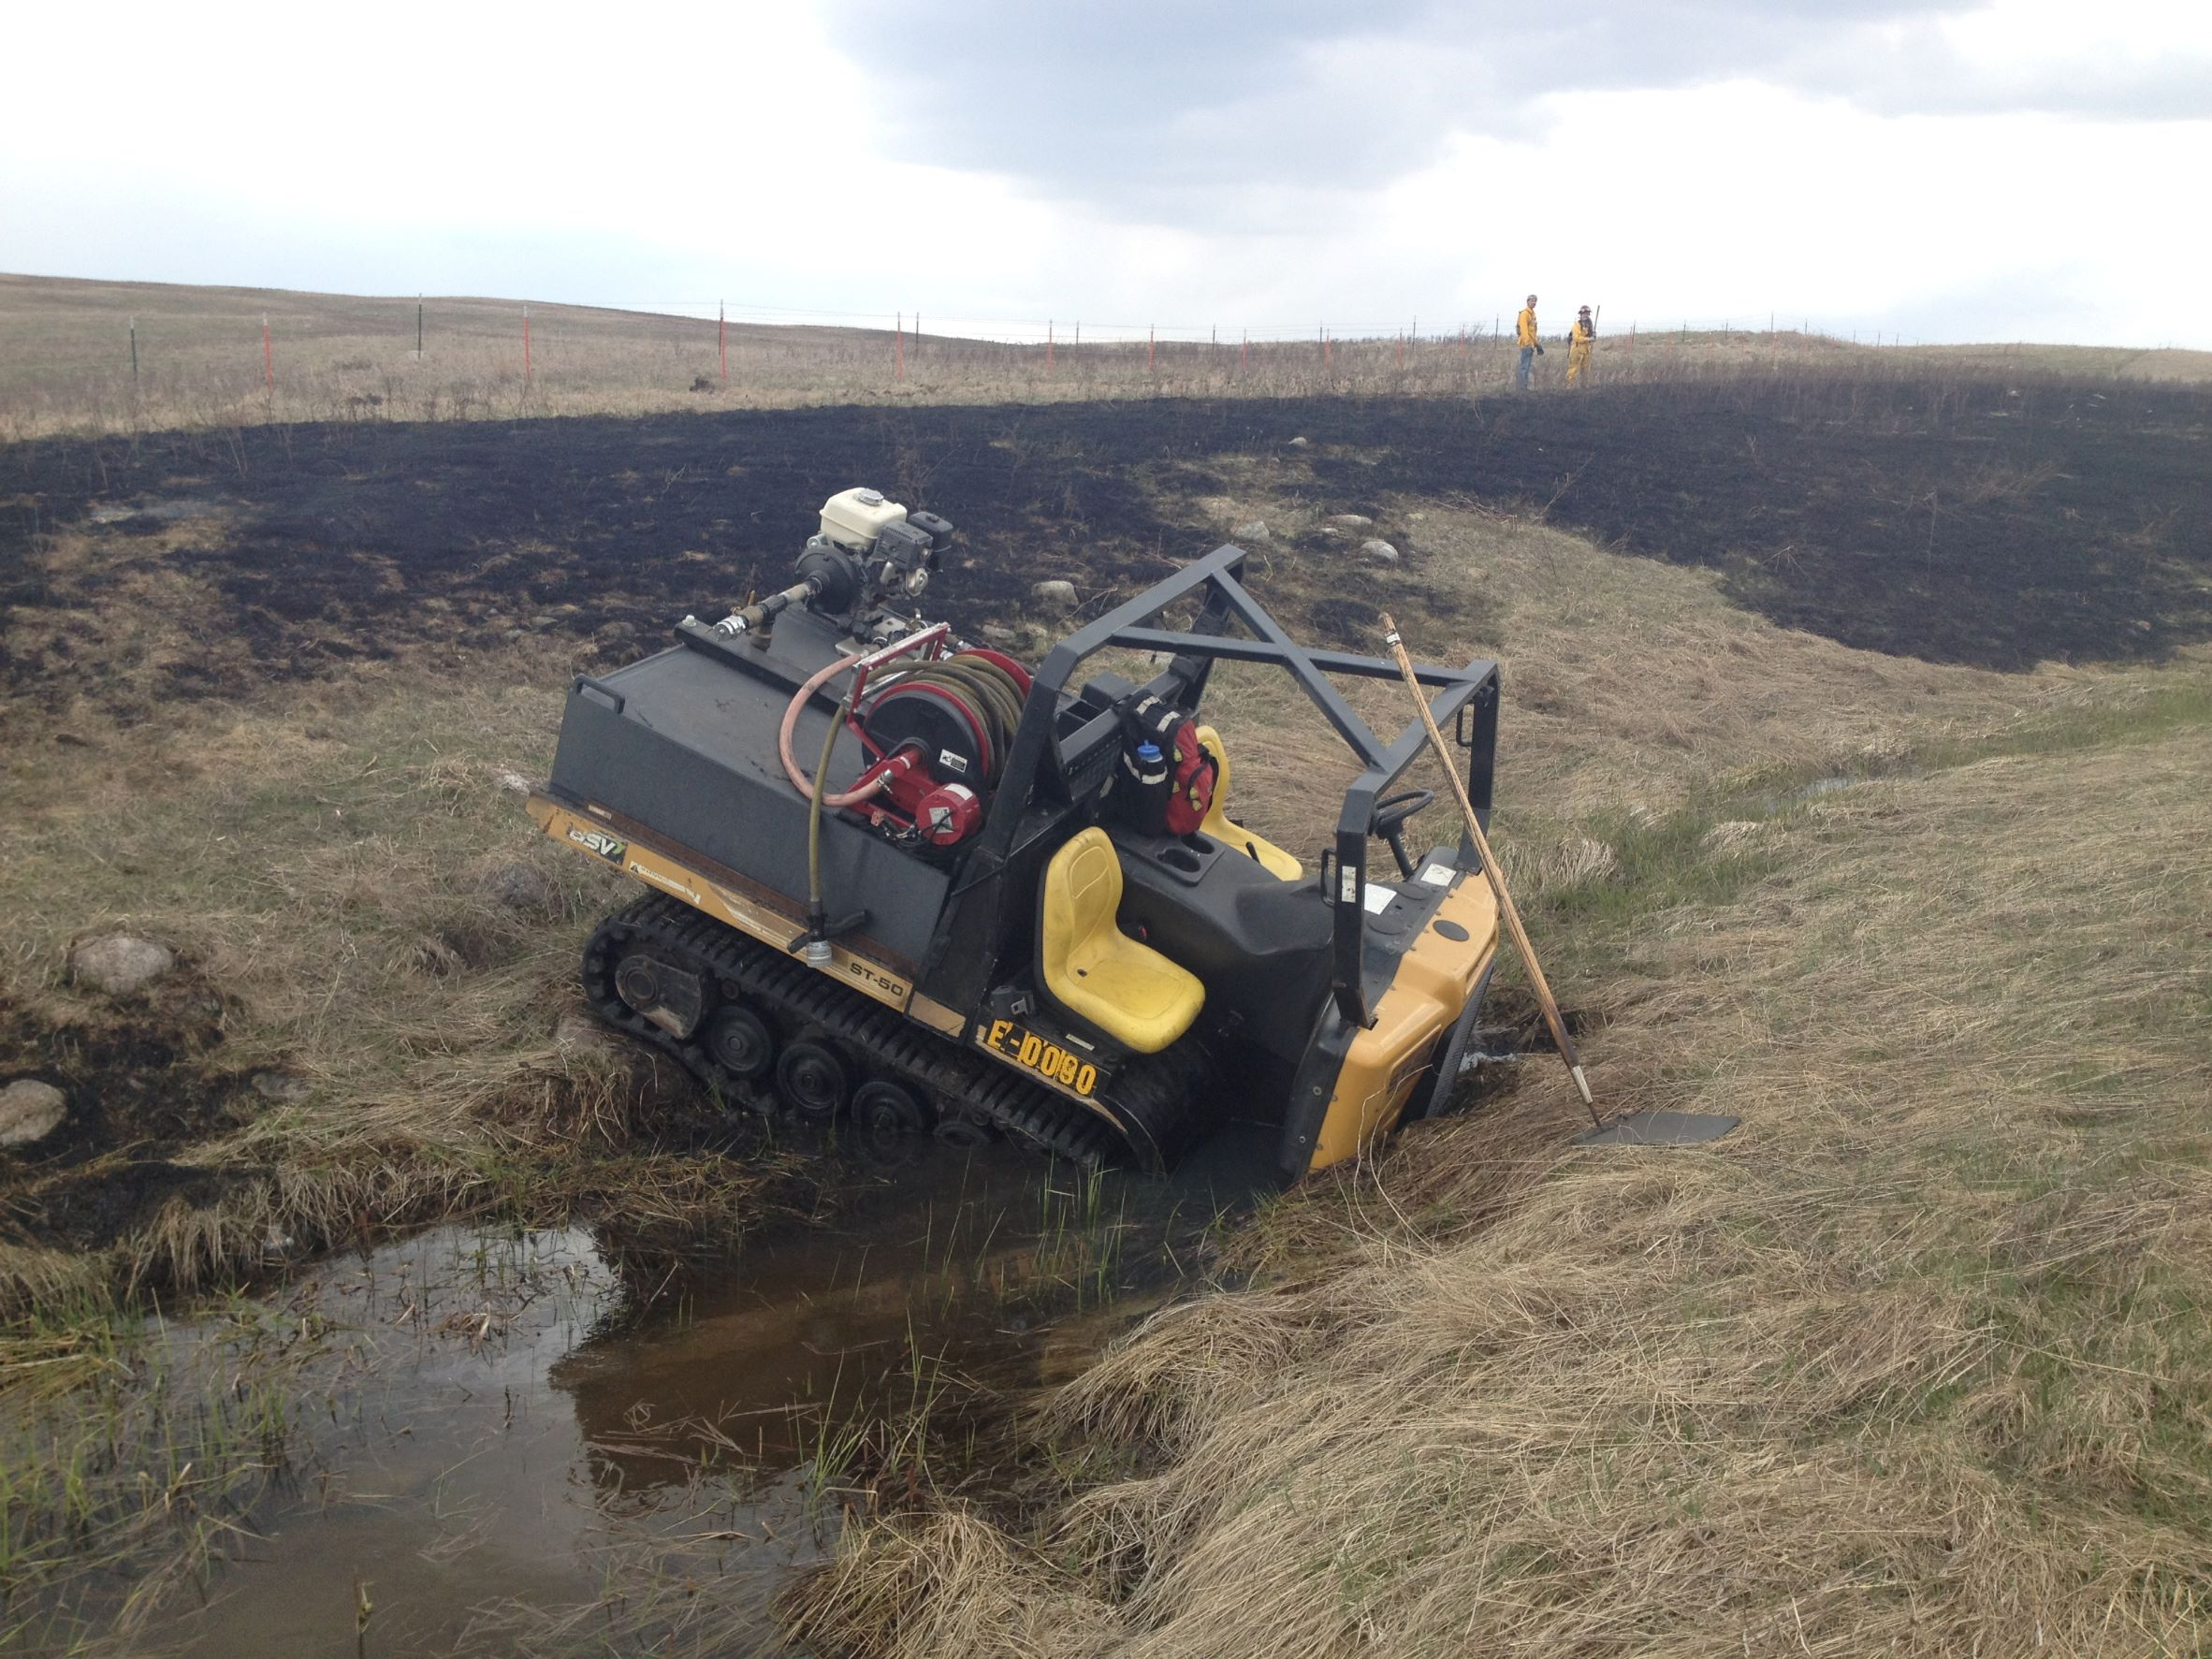
\includegraphics[width=2.2in]
		{ops/holding/ThorCreek}
		\caption{Sometimes it is best to just avoid the creek altogether.\label{fig:ThorCreek} } 
		% (Fig.~\ref{ThorCreek})
	\end{center}
\end{marginfigure} 

Existing roads make for excellent control lines (Fig.~\ref{fig:ReadyMadeBreaks}).
\emph{Slow fuel transitions} are another type of naturally-occurring or readymade fire break, defining the spatial threshold between flammable fuelbeds and low and/or green vegetation much less likely to carry fire (Fig.~\ref{fig:ReadyMadeBreaks}). 
Other areas of low flammability that can be incorporated into burn unit design include streams, rocky gulches, and outcroppings/ridges. 
When considering such features, it is important to consider both their tactical advantage\textemdash will a feature itself stop fire, or provide a good opportunity to burn out from with minimal preparation?\textemdash as well as their operational hazard\textemdash e.g., an uncrossable creek creates a level of complexity that managers can mitigate by putting line along the creek rather than across it (Fig.~\ref{fig:ThorCreek}). 

\subsection{Constructed line} 

\paragraph{Mineral lines}

The ideal line consists of \emph{mineral soil}\textemdash all vegetation is stripped away and the fire break is literally unable to burn such that no fire can creep across it.
In such cases, the degree of control provided by the line is limited only by its width\textemdash how long must flames be to lash across and ignite fuels outside the burn unit, and how long must embers smolder before they roll across and find receptive fuels. 

\begin{figure*} 
	\caption{\emph{Left \& center:} Wide mineral fire breaks constructed with farm tillage equipment make for robust control lines from which firing can be conducted with confidence.
		These lines in sw North Dakota were tilled through perennial grassland established on former crop fields (CRP), where damage to native sod and soil had already occurred.  
		\emph{Right:} In the Missouri Coteau, native prairie is often rocky, rolling, and invaded by the sod-forming Kentucky bluegrass, making for less reliable control lines that require frequent patrolling. 
	} \label{fig:MineralBreaks}
	\begin{center}
		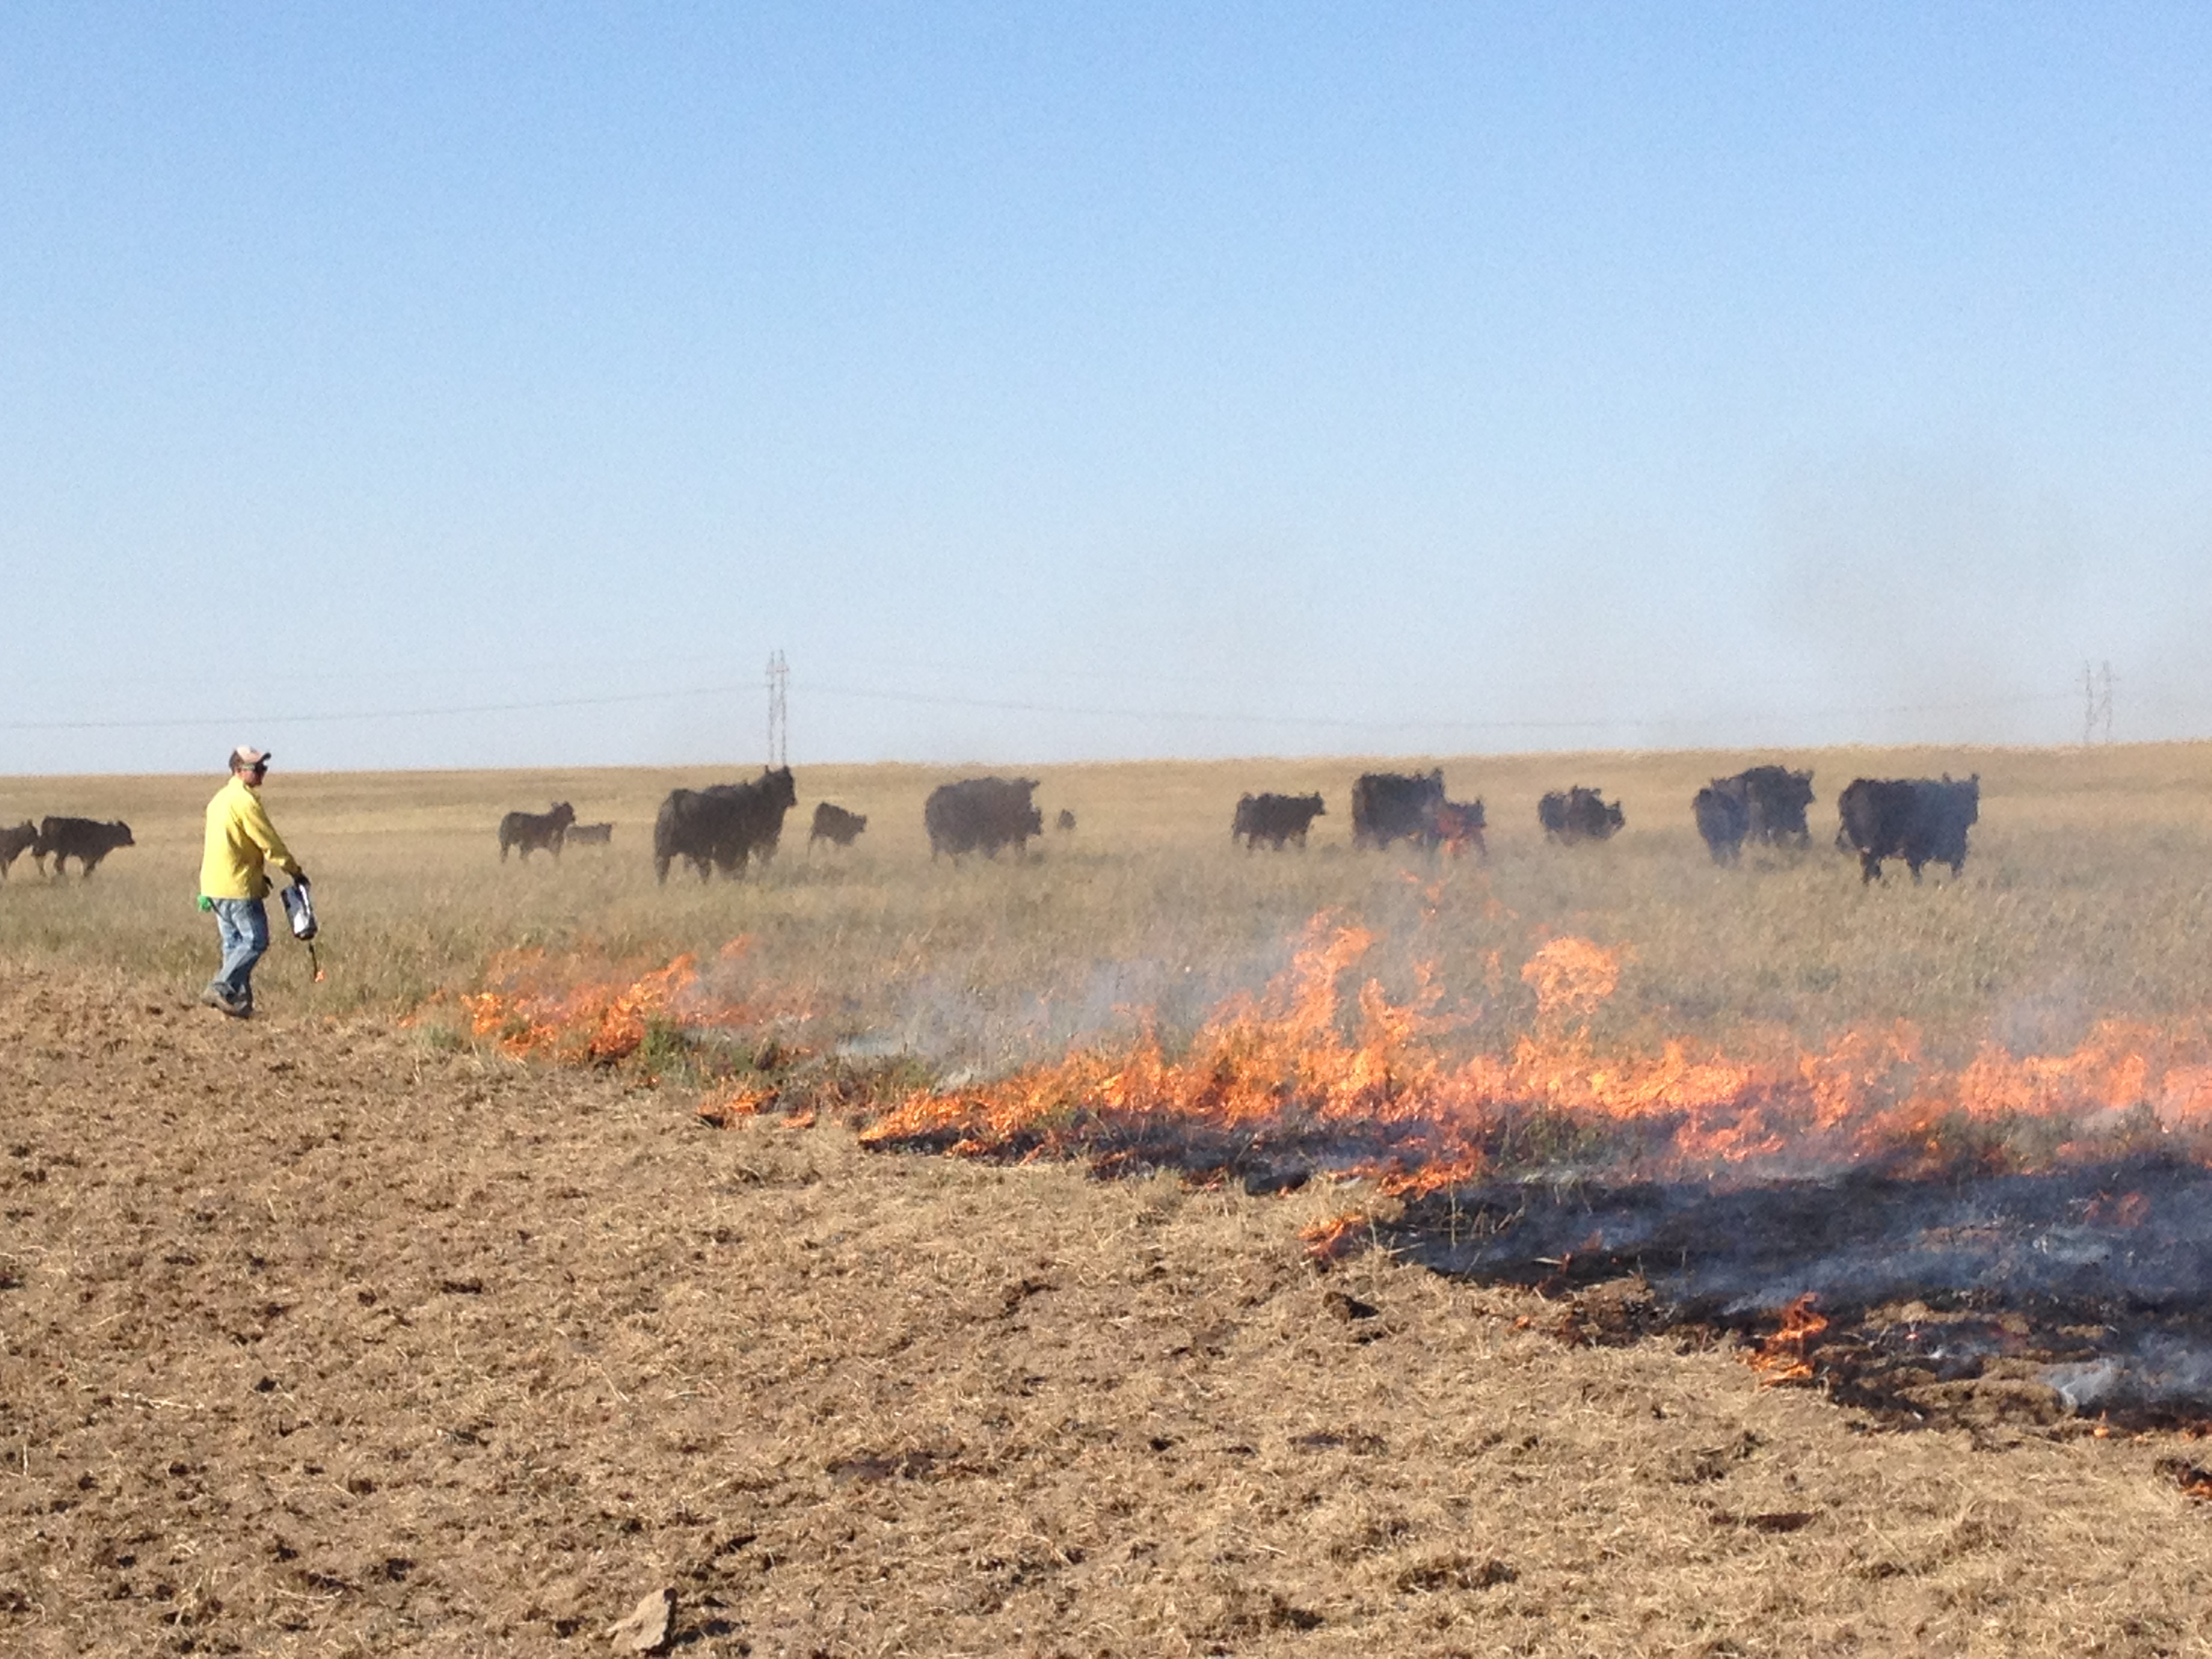
\includegraphics[width=0.33\textwidth]
		{ops/holding/MineralBreak}~
		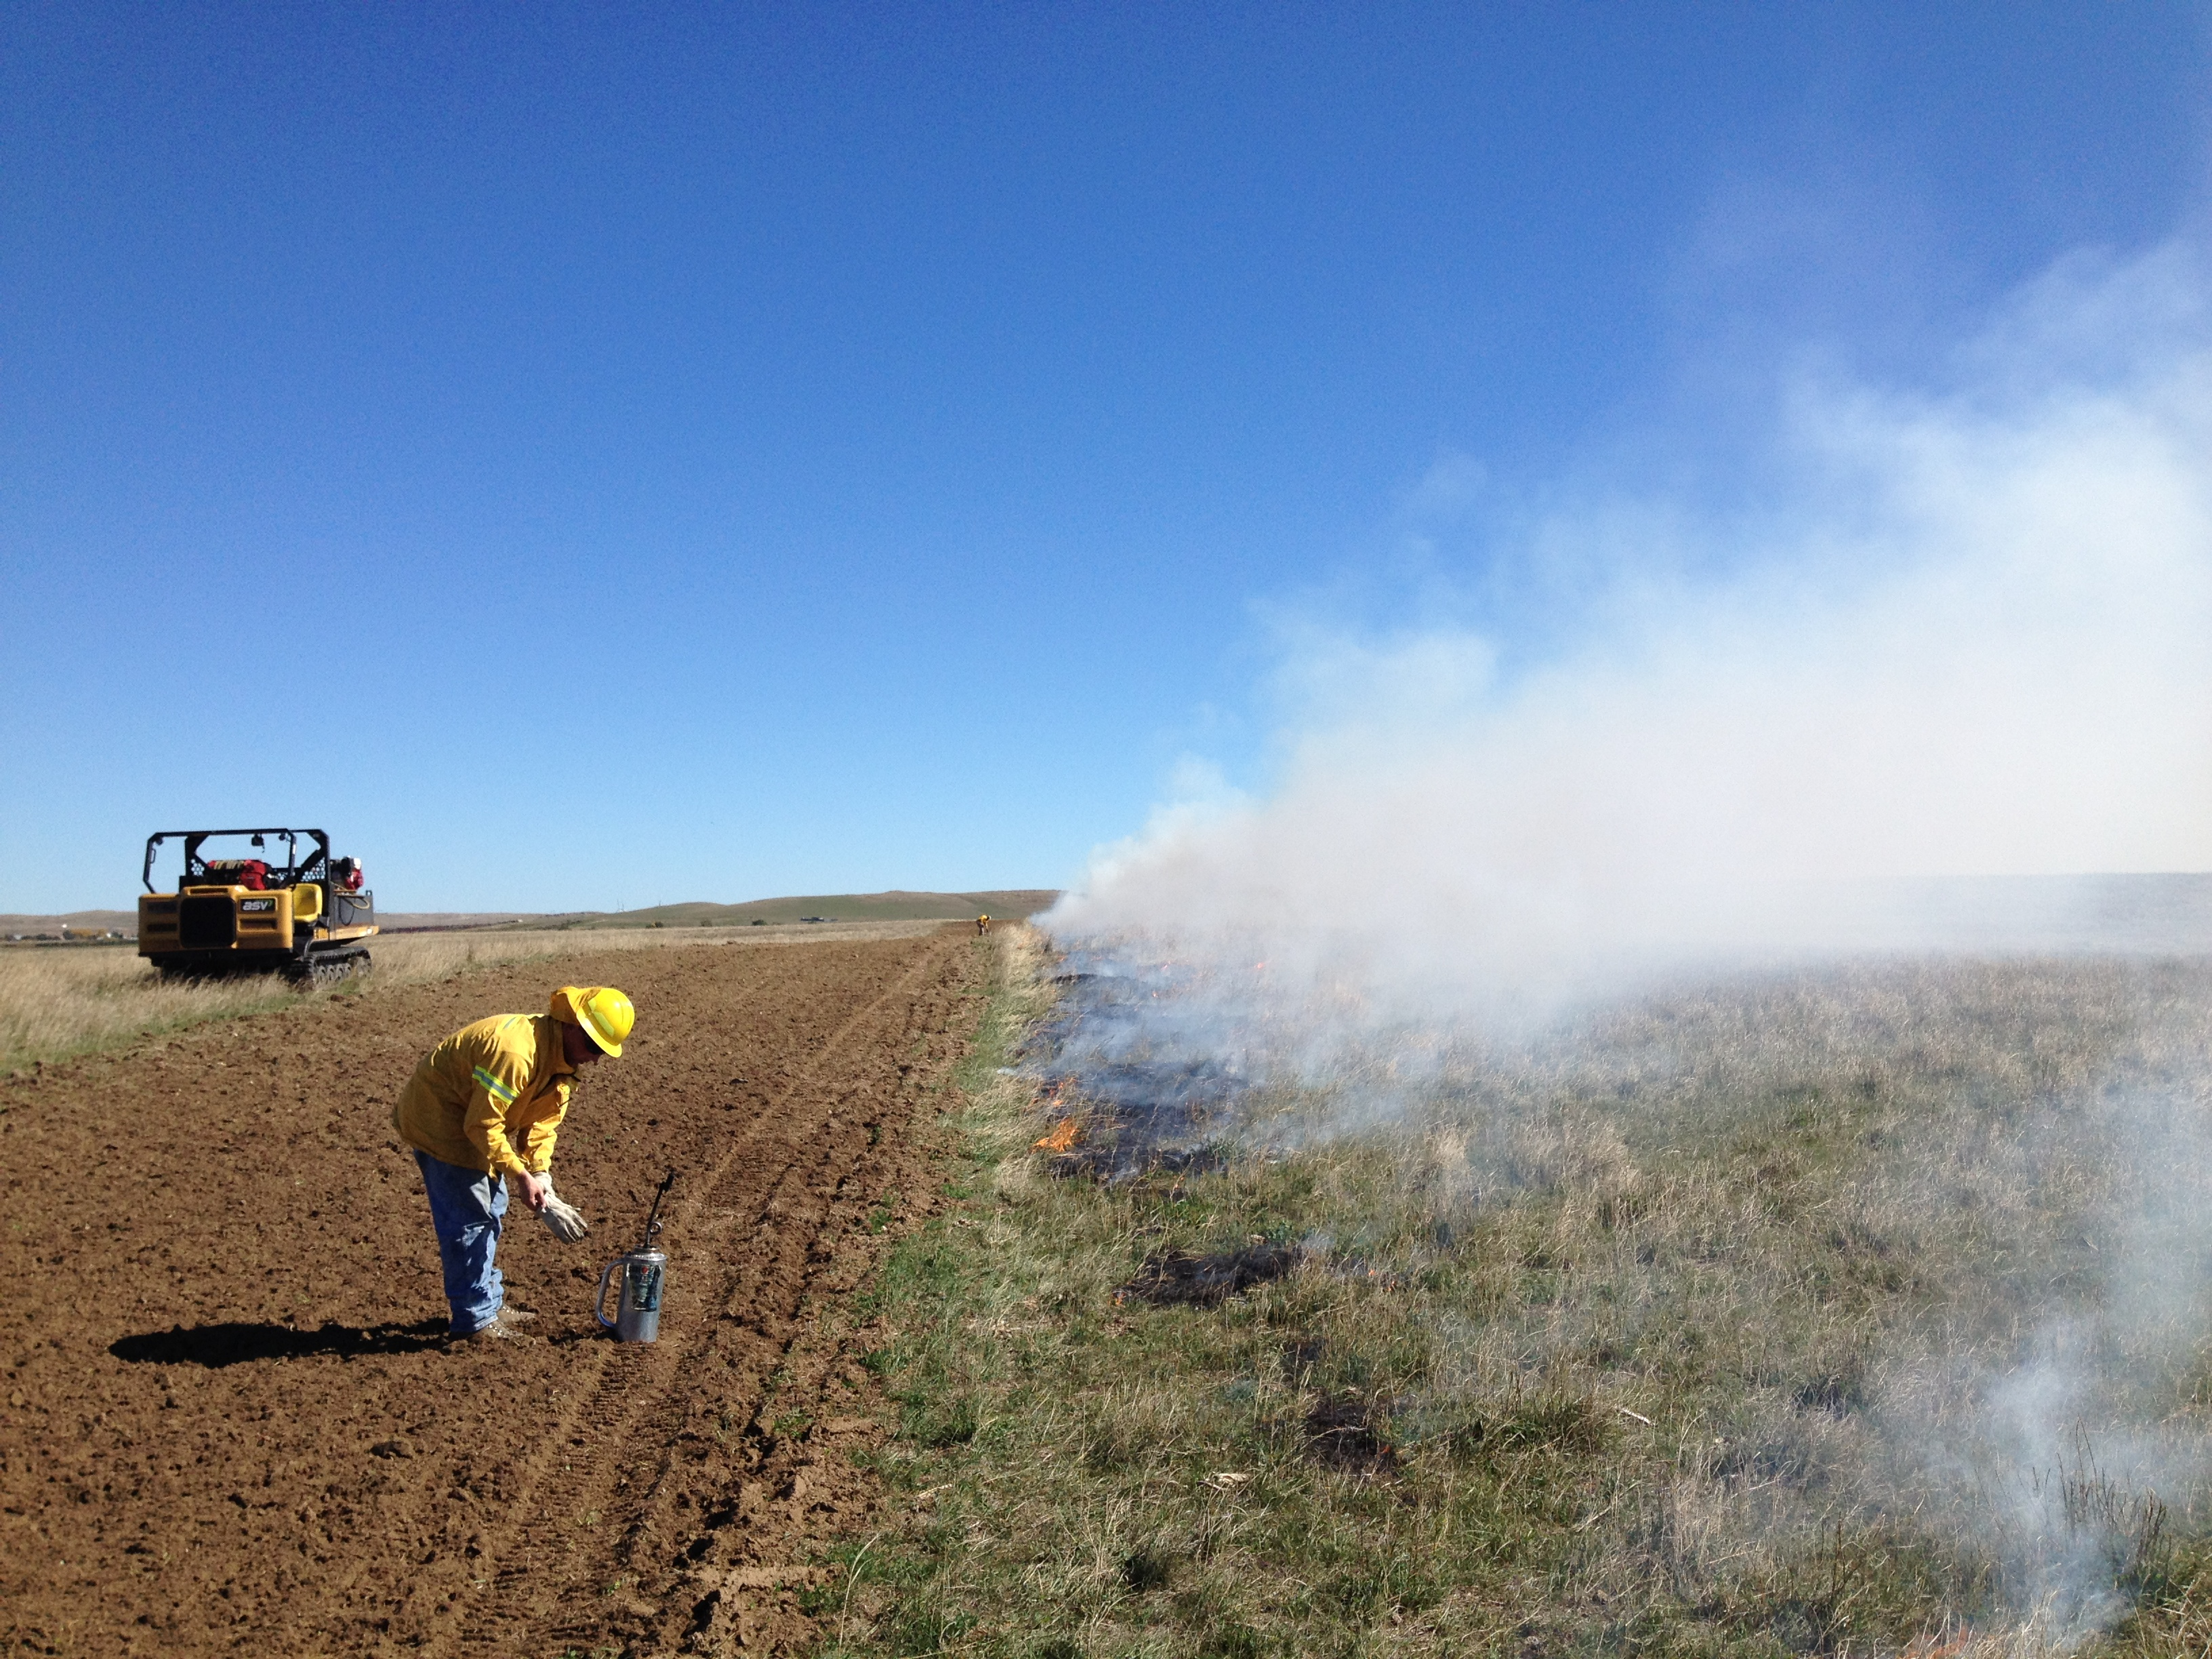
\includegraphics[width=0.33\textwidth]
		{ops/holding/WideMineralBreak2}~
		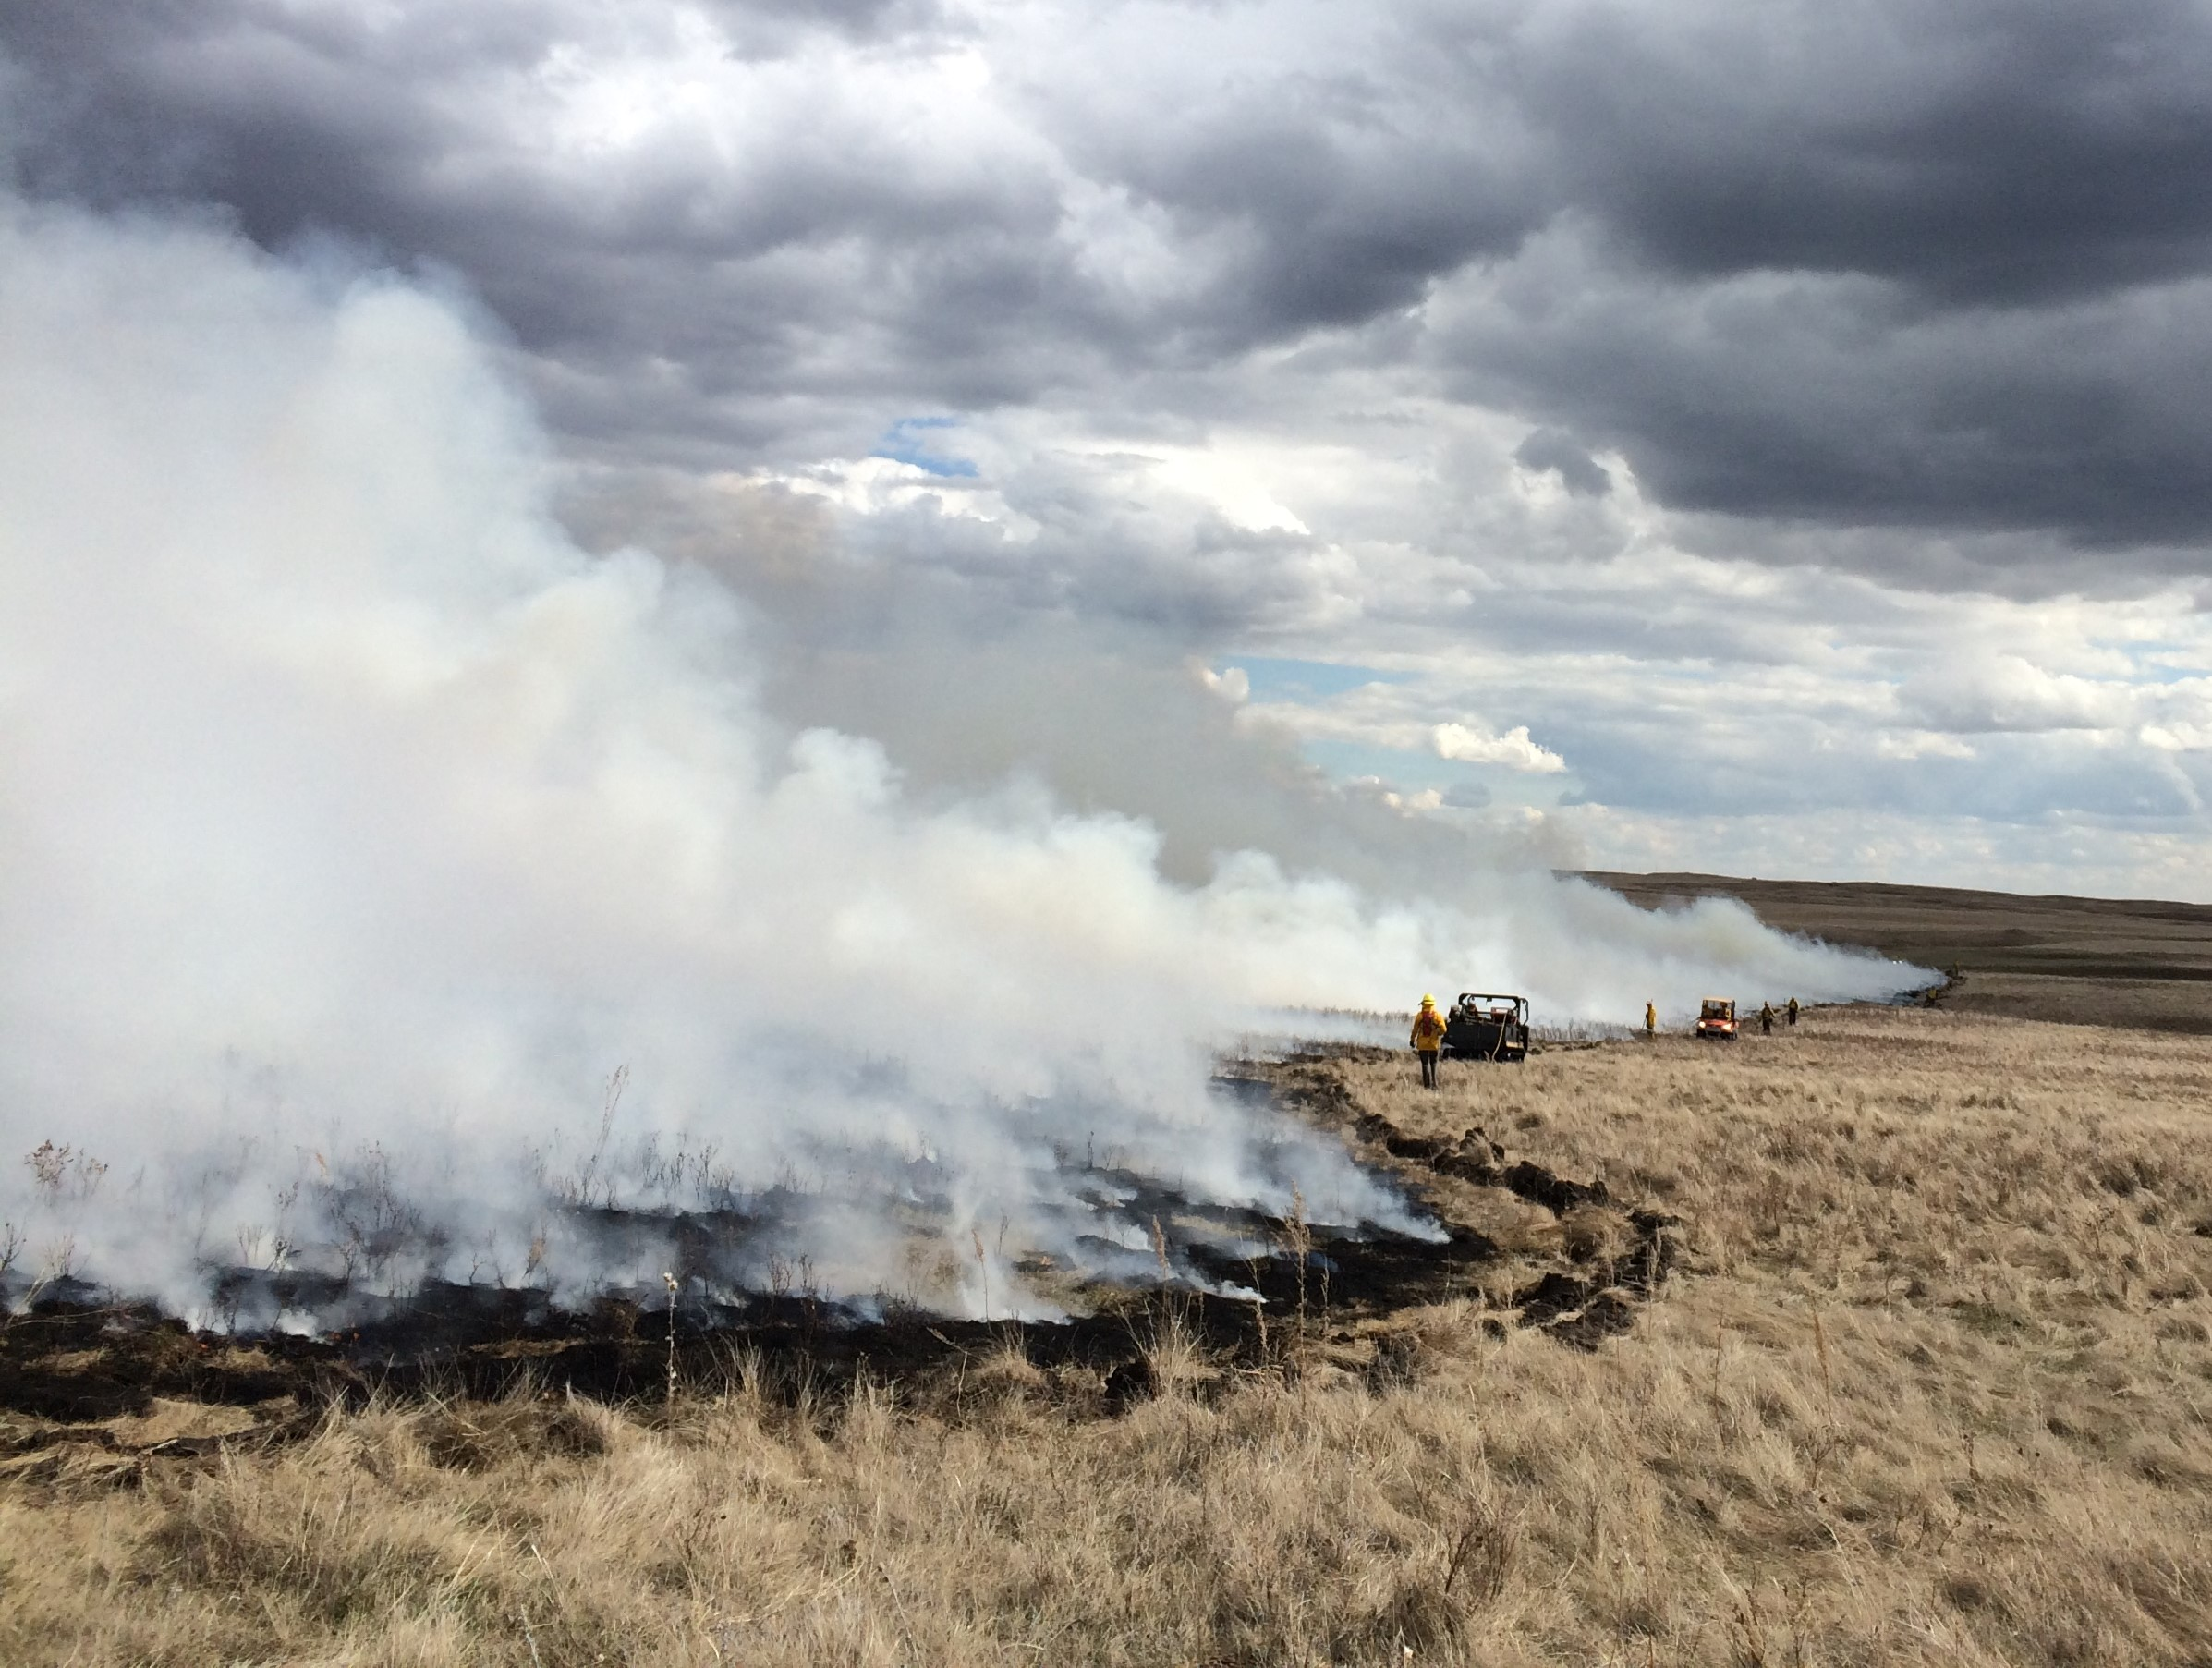
\includegraphics[width=0.33\textwidth]
		{ops/holding/SingleFurrow}
	\end{center}
	%(Fig.~\ref{fig:MineralBreaks})
\end{figure*}

Farm machinery is frequently implemented in constructing firebreaks for prescribed burns (Fig.~\ref{fig:MineralBreaks}). 
Generally speaking, tillage is more tenable on land currently or previously managed for agriculture\textemdash there is less concern about ``breaking virgin prairie''. 
Thus, wider lines that provide a high degree of control are possible when the terrain is conducive to wide tillage equipment (Fig.~\ref{fig:MineralBreaks}, \emph{left \& center}). 
But terrain and concerns about soil disturbance impact often limit mineral lines to a single furrow, which can be much more difficult to control, especially in vegetation types that form dense sod (Fig.~\ref{fig:MineralBreaks}, \emph{right}). 

\paragraph{Mowed fire breaks}

When tillage is not an option, mowing is a standard approach to creating lines of low fuels in which fire is much more easily controlled (Fig.~\ref{fig:MowedBreaks}). 
Rather than being non-combustible, mowed breaks are expected to burn to some degree, but fire is extinguished on the border of the unit as the black widens. 
Turning mowed lines cold is much more easily done when mowed vegetation is removed after cutting, which essentially creates a dense layer of fully-cured fine fuels. 
In many areas, frequent mowing tends to shift vegetation towards a generally less-flammable community dominated by sod-forming species. 
At the same time, these species also tend to be non-native; the ecological after-effects of fireline construction and maintenance must be considered alongside the ecological benefits of prescribed fire. 

\begin{figure} 
	\begin{center}
		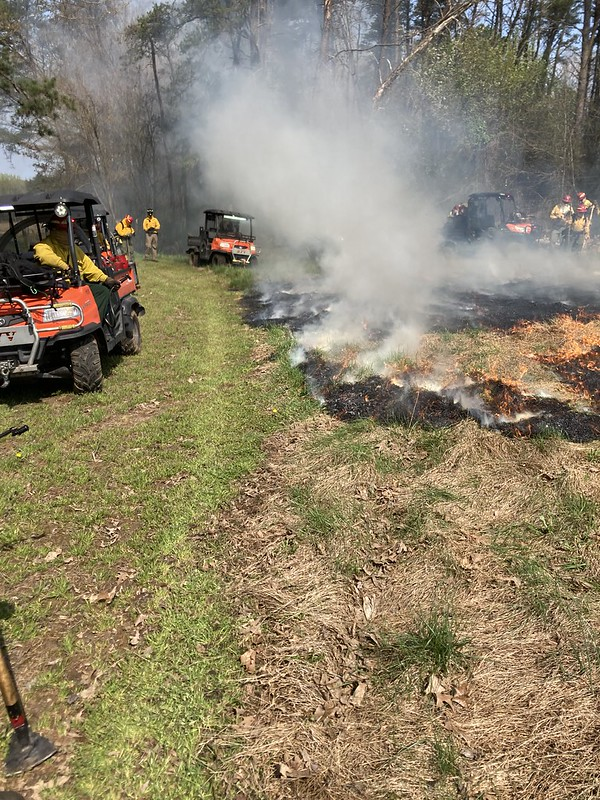
\includegraphics[width=0.36\textwidth]
		{ops/holding/GreenMowedLine}~
		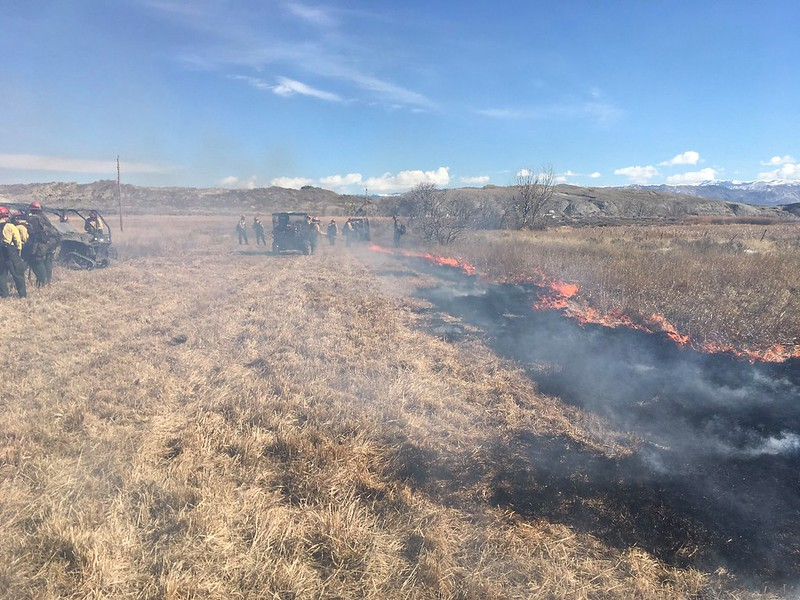
\includegraphics[width=0.64\textwidth]
		{ops/holding/MowedLineBreak}
	\end{center}
	\caption{When tillage to mineral soil is not an option, reducing fuel loads by mowing is a good option. 
		Mowed breaks are most effective when fuel removal is complemented by a slow-fuel transition, such as green, sod-forming grass along frequently-mowed trails (L). 
		Otherwise, fire can still spread through remaining dry stubble, although lower flame lengths facilitate control (R). 
		Note the undulating black line on the right, reflecting the fact that backing fires needed to be suppressed, and didn't go out on their own upon encountering lower fuel loads.   
	} \label{fig:MowedBreaks}
	%(Fig.~\ref{fig:MowedBreaks})
\end{figure}

\paragraph{Hand line}

When machinery is simply not an option, hand labor can create control lines. 
This is a conventional approach in indirect attack in wildfire suppression; hand crews dig narrow mineral lines from which ignitions specialists burn out to create wide control lines (Fig.~\ref{fig:Handlines}). 
Although it requires more physical effort than most prescribed fire managers prefer to exert for an extended period, hand line can be deployed to ``tie in'' gaps in fire breaks that machinery could not reach, or to create small defensible spaces within burn units (e.g., around power poles and structures). 
In woodlands and savannas where surface fuels are dominated by leaf litter, hand lines are easily constructed with rakes and leaf blowers (Fig.~\ref{fig:leaflines}). 

 \begin{marginfigure}[-4cm]
	\begin{center}
		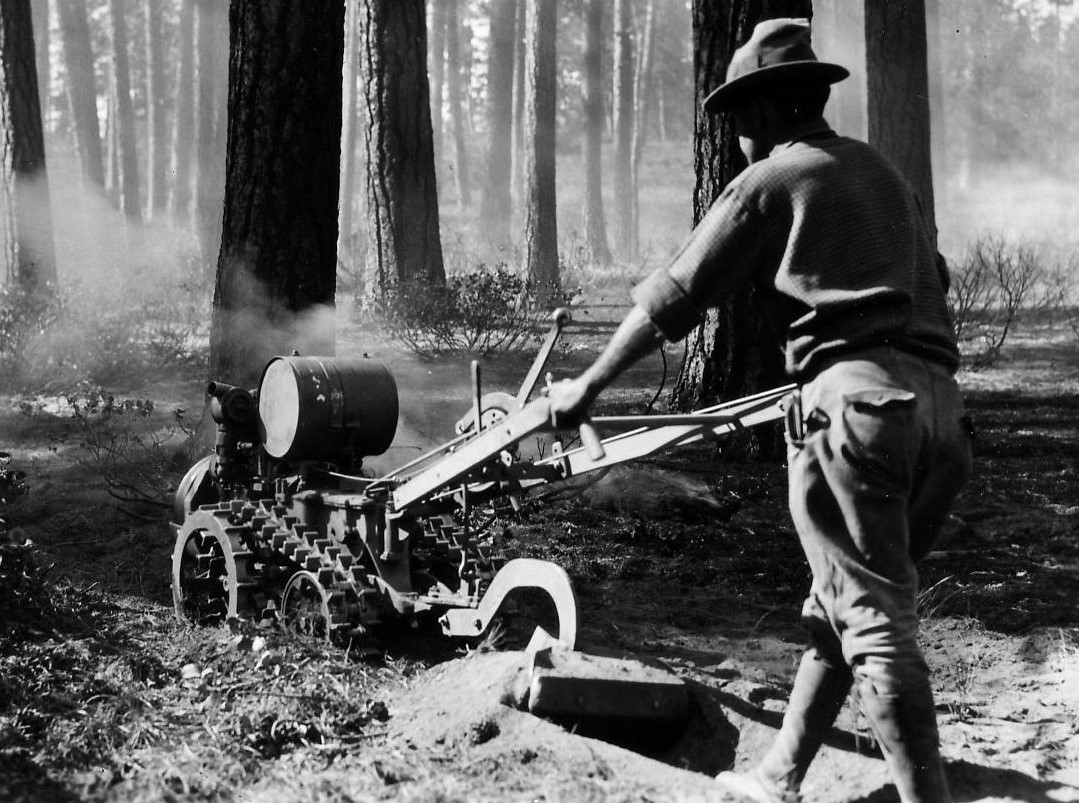
\includegraphics[width=2.2in]
		{ops/holding/Rototiller}
		\\
	{Fortunately machinery has evolved since internal combustion engines were first applied to digging fire line. } 
		% (Fig.~\ref{fig:groundhog})
	\end{center}
\end{marginfigure}

\begin{figure} 
	\begin{center}
		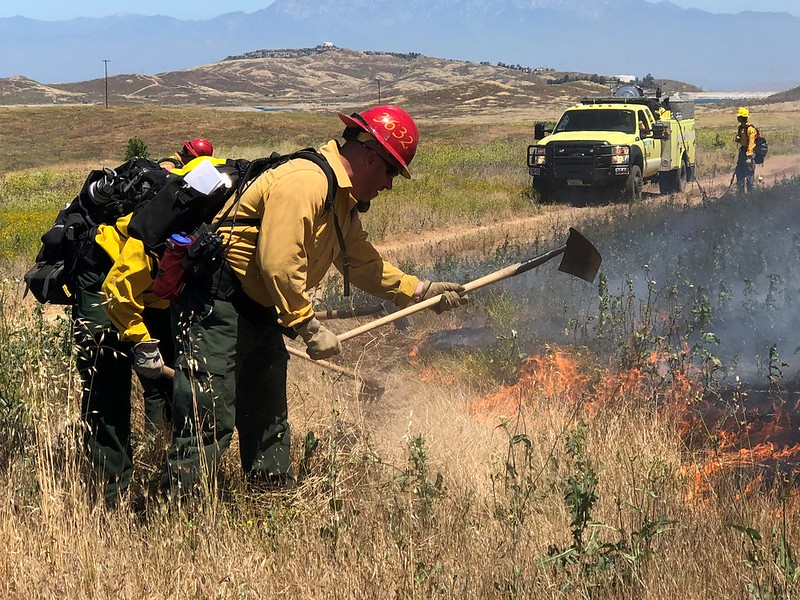
\includegraphics[width=0.47\textwidth]
		{ops/holding/RxFireHandline}~
		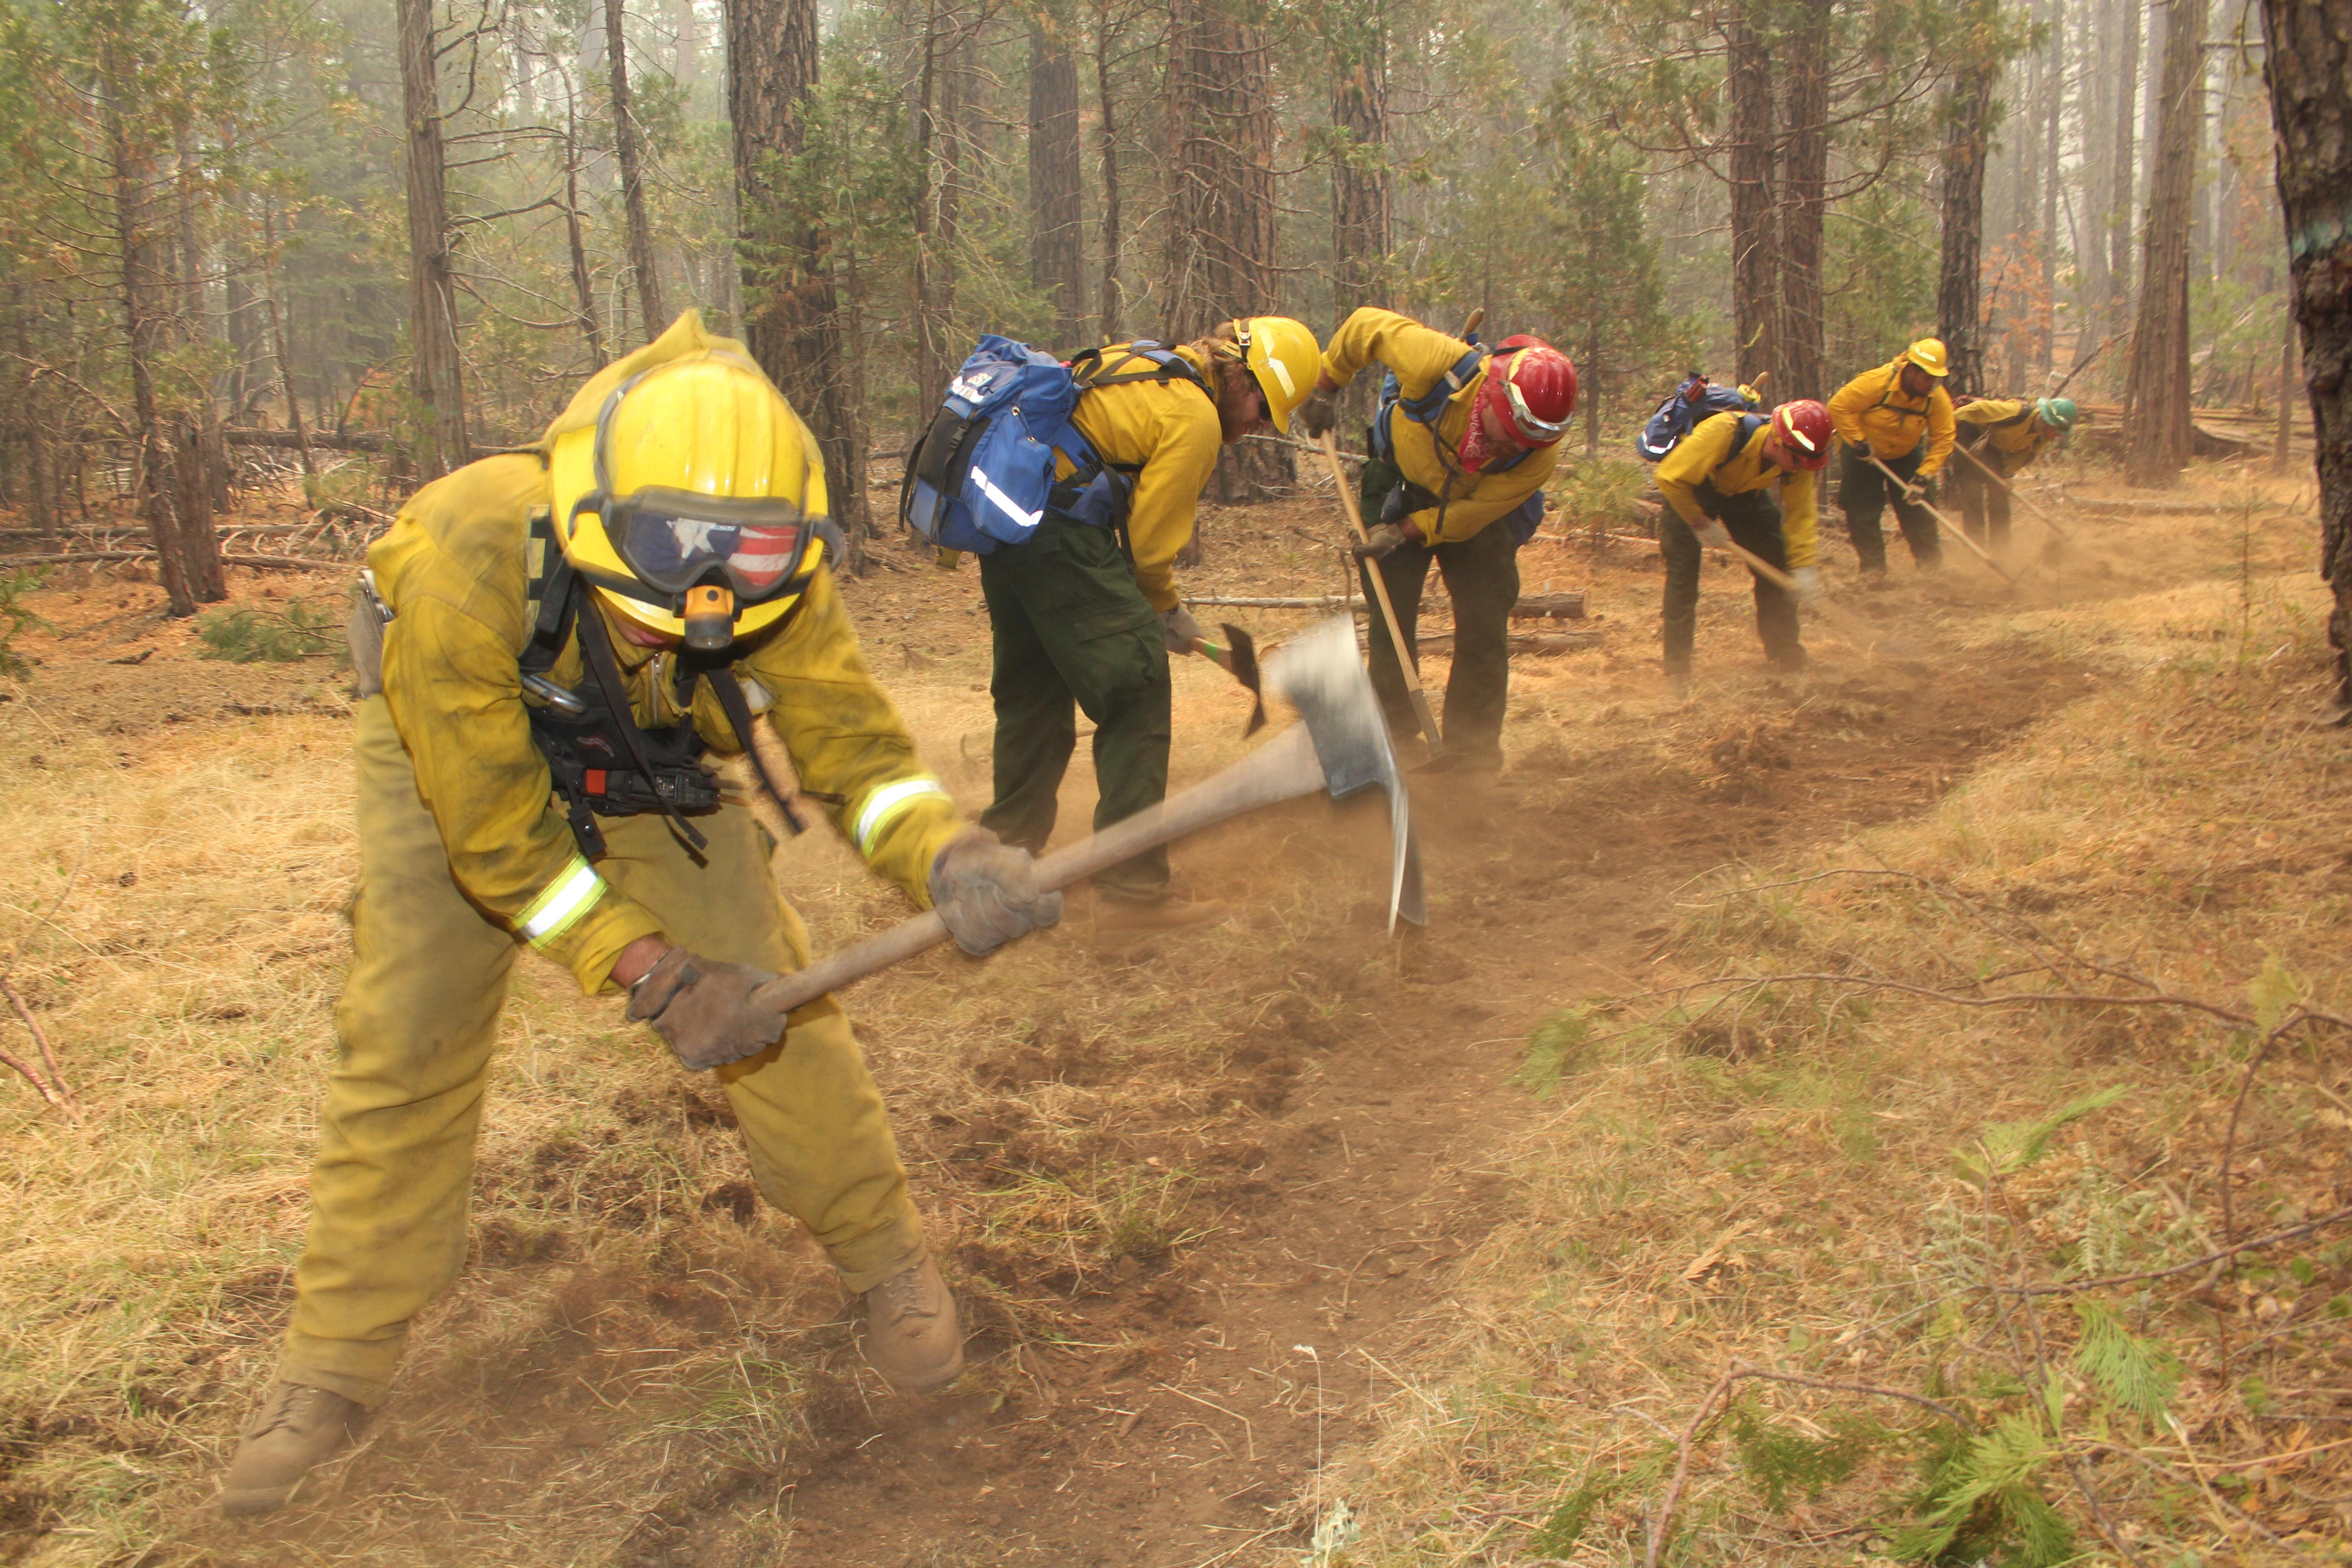
\includegraphics[width=0.53\textwidth]
		{ops/holding/HandCrew}
	\end{center}
	\caption{When machinery can't reach locations that don't have usable natural fire breaks, crews with hand tools can attack the flame front directly (L) or support indirect attack by constructing line by hand (R). 
		The end goal is to remove vegetation down to mineral soil, often providing a point from which to begin backburning. 
	} \label{fig:Handlines}
	%(Fig.~\ref{fig:Handlines})
\end{figure}



\begin{figure} 
	\begin{center}
		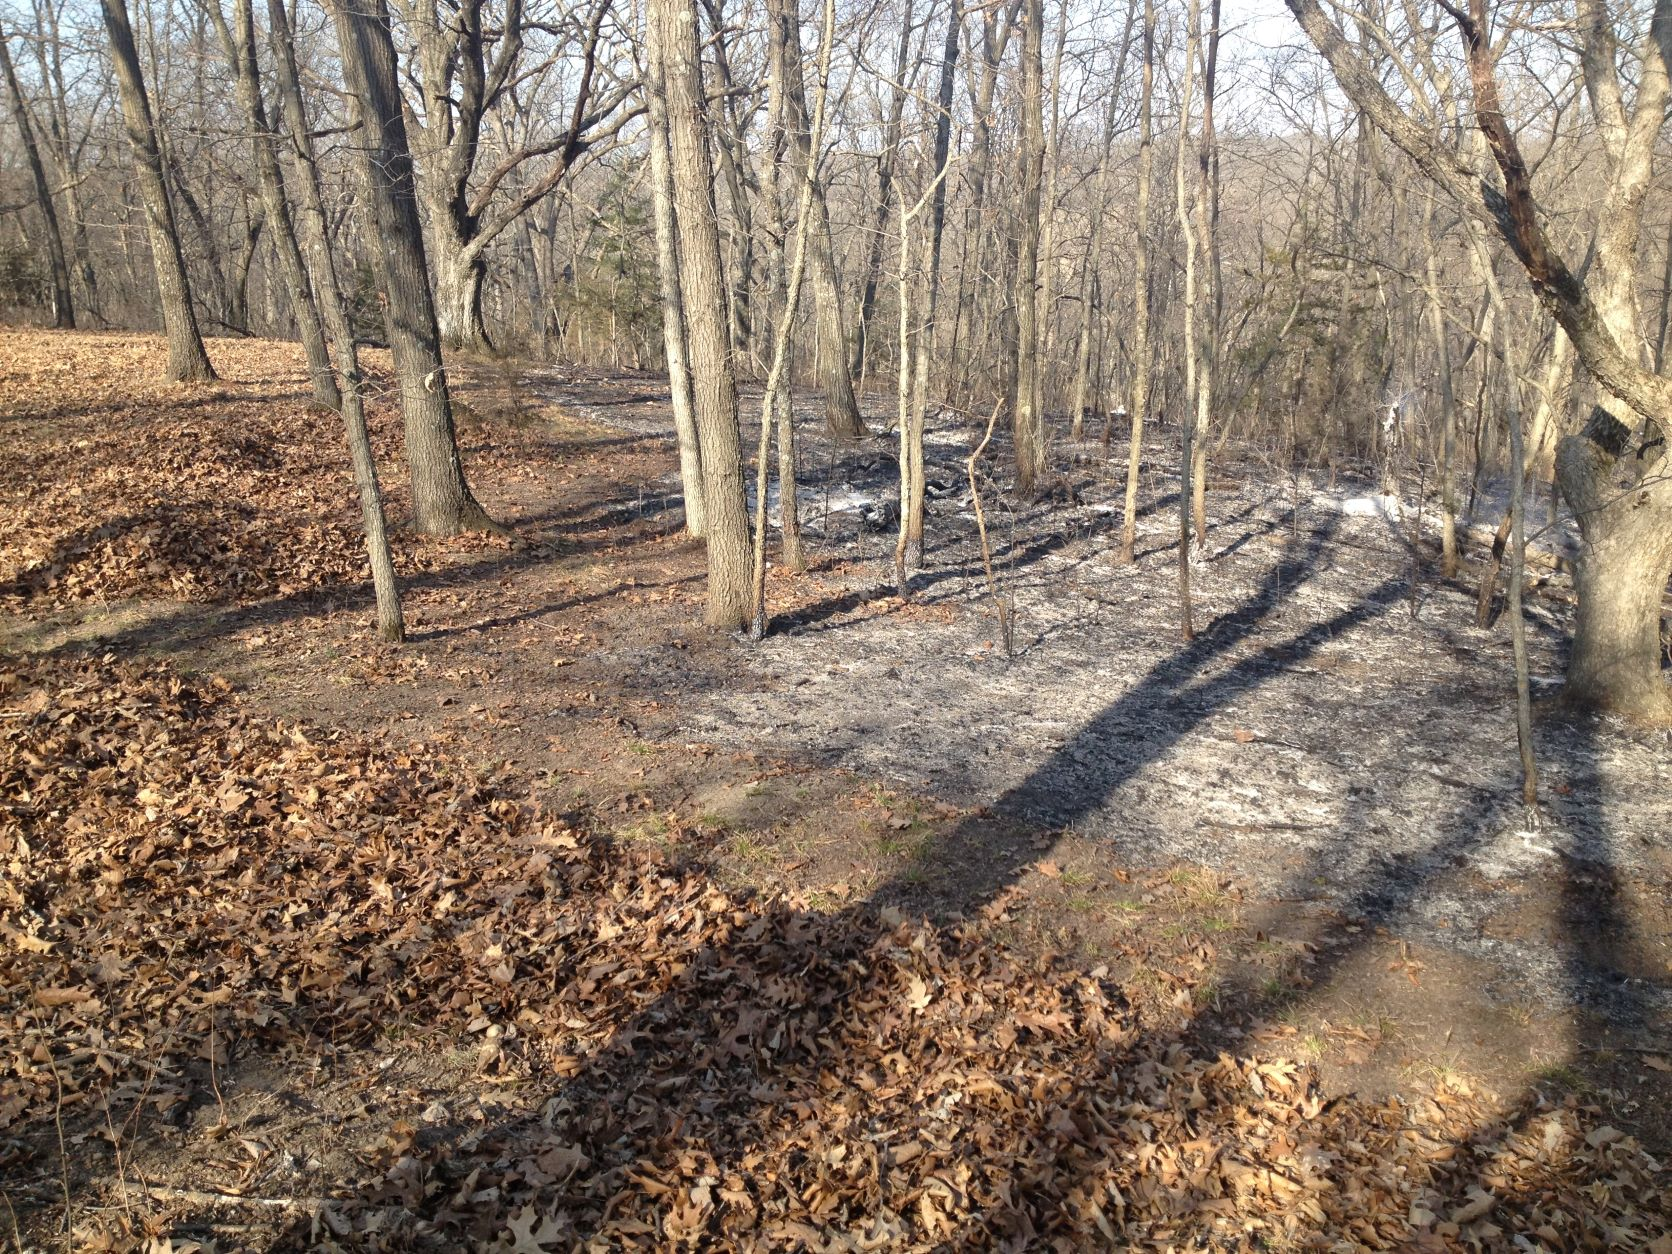
\includegraphics[width=0.5\textwidth]
		{ops/holding/OakLeafBreak1}~
		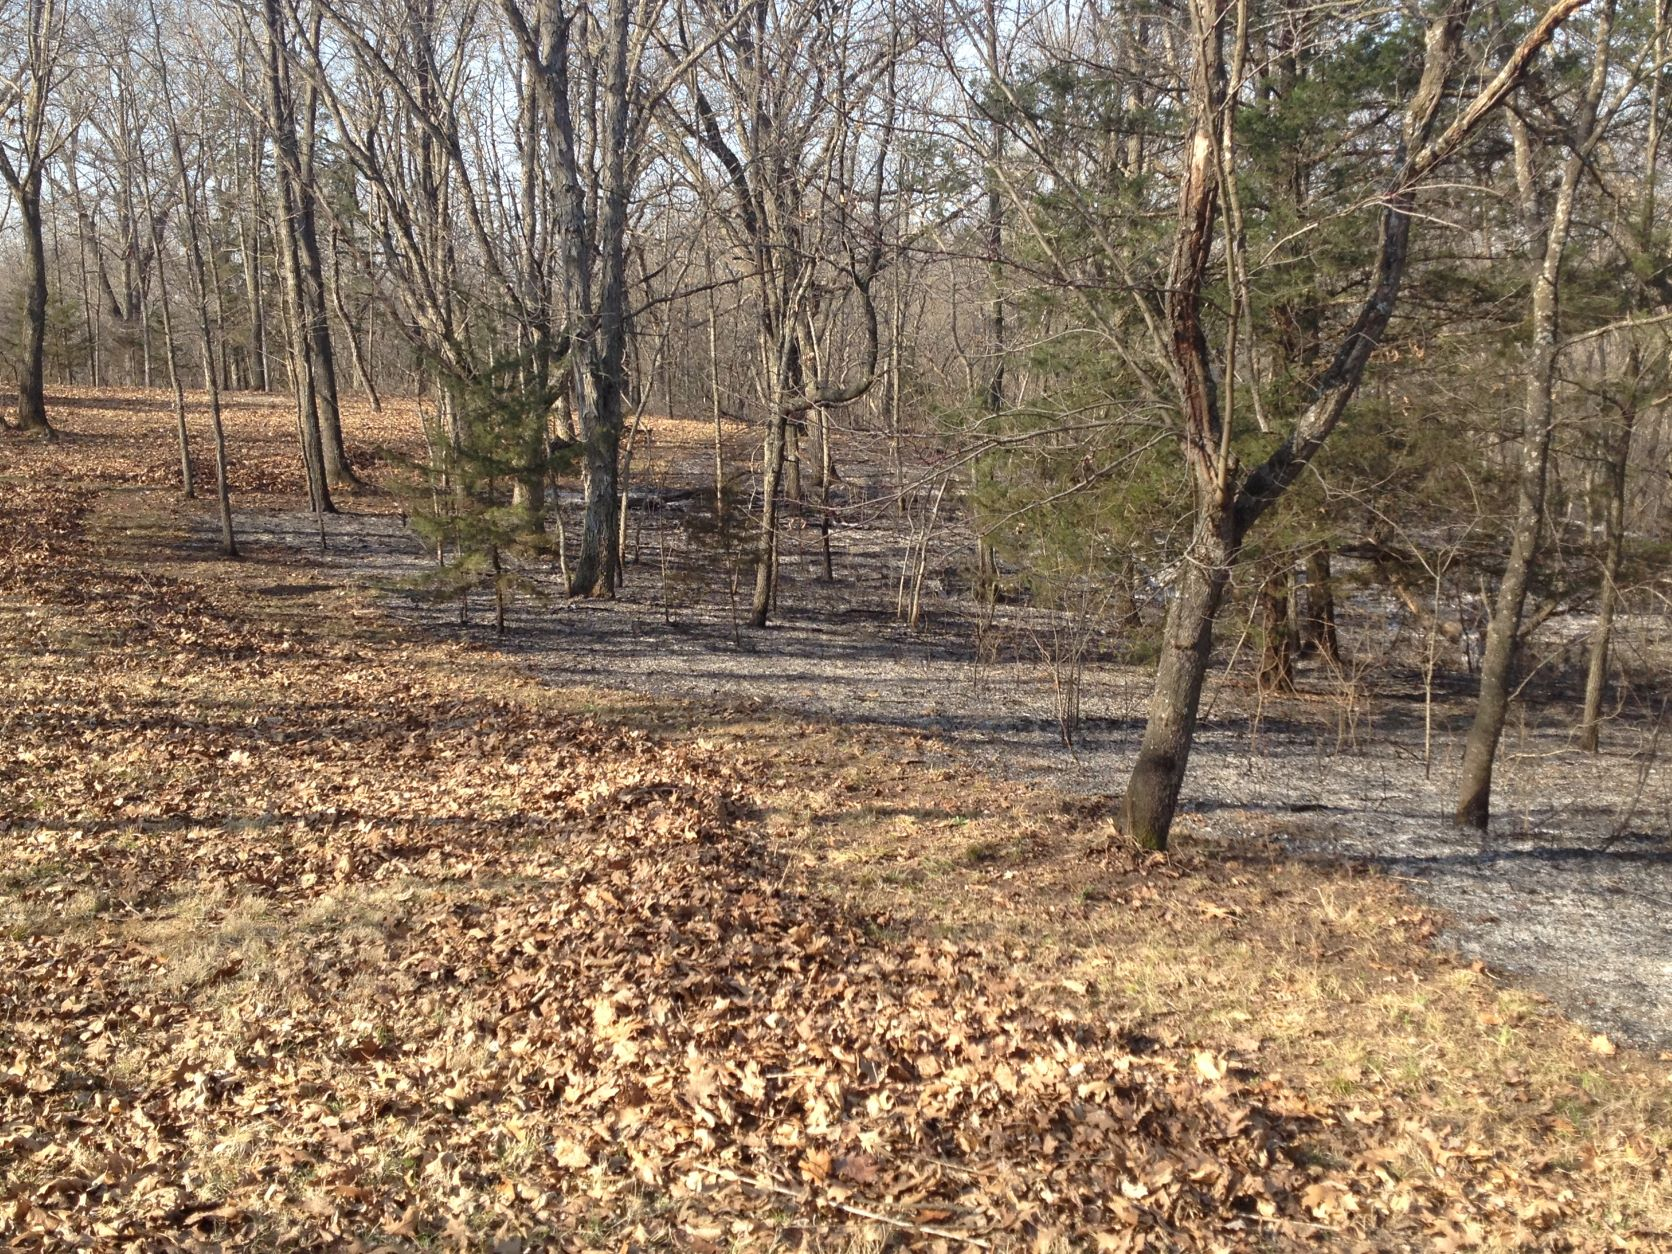
\includegraphics[width=0.5\textwidth]
		{ops/holding/OakLeafBreak2}
	\end{center}
	\caption{These control lines in hardwood-dominated woodland outside Lawrence, Kansas were put in by the landowner with rakes and a leafblower.  
	} \label{fig:leaflines}
	%(Fig.~\ref{fig:leaflines})
\end{figure}

\section{Control tactics} 

It is essential that prescribed fire managers be prepared to control their fire. 
Crew members might need to take suppressive action in response to a spot fire or  \emph{slop over}\textemdash when fire manages to cross a control line and burn where it shouldn't\textemdash when the fire \emph{escapes}\textemdash i.e., begins to spread through a neighboring property not part of the burn unit\textemdash and simply when primary torch lines have served their purpose and no longer need to be burning at the edge of the unit. 

When flames are about 3 ft long or less, properly equipped and trained personnel  can attack directly using hand tools typical of a prescribed fire holding crew (e.g., flappers and rakes). 
Even then, fires ought to be engaged from control lines or the black. 
When flames are much longer than 3 ft, under no circumstances should anyone attack the fire directly with a hand tool. 
Such fires ought only to be engaged along the flanks, from the black, and with water\textemdash the radiant heat is just too intense to work near the fire even if wind is moving convective heat away. 

 \begin{marginfigure}
	\begin{center}
		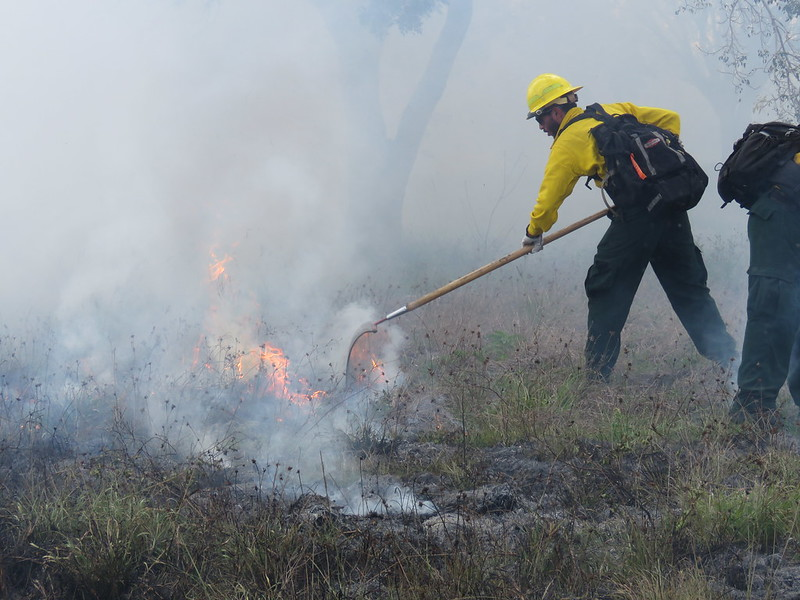
\includegraphics[width=2.2in]
		{ops/holding/FlapperInSmoke}
		\caption{A holding crew member works to smother flames with a flapper. 
		\label{fig:flapper}  } 
		% (Fig.~\ref{fig:flapper})
	\end{center}
\end{marginfigure}

The primary objective of hand tools is to deprive a flame front of one or more sides of the flame triangle (Fig.~\ref{fig:FireTriangles}).  
For example, flappers are designed to smother the fire by denying oxygen to the reaction zone (hence the adage ``don't flap a flapper,'' which risks fanning the flames instead of smushing them out; Fig.~\ref{fig:flapper}). 
When properly used to reach ahead of the flame front and drag material back into the black, rakes remove fuel. 
In fine fuels, all of these interventions provide ample time for the reaction zone to cool, such that even if access to oxygen is restored, there is insufficient heat for combustion to occur. 







